%%%% CAPÍTULO 3 - MATERIAL E MÉTODOS (PODE SER OUTRO TÍTULO DE ACORDO COM O TRABALHO REALIZADO)
%%
%% Deve apresentar o modelo utilizado, a modelagem
%% empregada, as simplificações necessárias, a
%% metodologia e a descrição do método de cálculo 
%% utilizado no desenvolvimento da pesquisa para que
%% a mesma possa ser reconstituída. Deve ainda 
%% apresentar resultados de amostras e comentários.
%% Deve apresentar a descrição da montagem 
%% experimental, metodologia para a obtenção de 
%% resultados, análise de erros, amostra de resultados
%% obtidos e comentários. Atenção: Esta parte pode ser
%% subdividida em mais capítulos de acordo com a 
%% especificidade do assunto.

%% Título e rótulo de capítulo (rótulos não devem conter caracteres especiais, acentuados ou cedilha)
\chapter{Software}\label{cap:materialemetodos}

\section{Ferramentas e Bibliotecas}
O código do controlador foi feito utilizando o IDE do arduino e as bibliotecas "MPU6050\textunderscore light" e "Servo", disponíveis para download pelo IDE. A primeira biblioteca realiza a leitura dos sensores acelerômetro e giroscópio pelo barramento I2C do arduino, além de combiná-los com um filtro complementar que será explicado a seguir. A segunda biblioteca realiza o controle das posições dos servo motores por meio de um sinal PWM. Uma visão geral do funcionamento do sistema é dada pelo fluxograma na figura 7.

\begin{figure}[H]
\centering
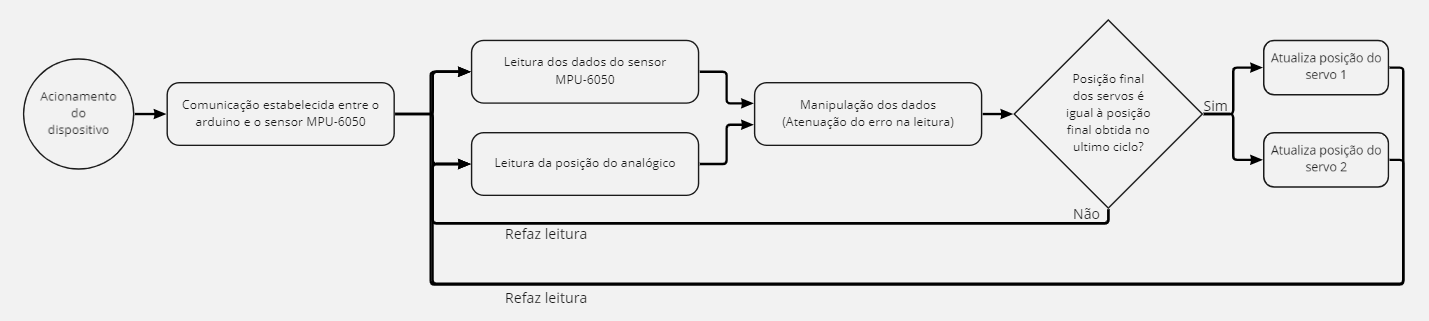
\includegraphics[width=1\textwidth]{Capitulo3 - Software/Fluxograma.png}\\
\caption{\label{fig:widgets}Fluxograma da sequencia de operação do sistema.}
\end{figure}

\section{Ângulos a partir das leituras do MPU-6050}
A leitura dos sensores é realizada pela biblioteca "MPU6050\textunderscore light", são lidos utilizando o protocolo I2C os valores brutos da aceleração linear, do acelerômetro, e angular, do giroscópio.\\
\indent Em funcionamento normal a maior aceleração linear percebida pelo dispositivo é a gravidade e, com um pouco de trigonometria, é calculada a rotação do sistema em relação à direção "para baixo". Ao longo do tempo o valor médio calculado se mantém próximo do esperado, porém qualquer movimento, até mesmo as vibrações de origem térmica no material, causam ruídos e ainda não podemos utilizar essa leitura diretamente.\\
\indent Das leituras da aceleração angular podemos integrar o sinal duas vezes para obter a velocidade angular e então o ângulo relativo à alguma posição de referência. Para um tempo curto essa leitura já basta, contudo o erro do sistema é somado em cada ciclo de integração e um desvio vai se acumulando com o tempo. Outro problema que precisa ser corrigido antes de utilizar essa leitura é a definição dessa posição de referência.\\
\\
\indent Pode-se observar então que temos uma variável com boa confiança em curto prazo (do giroscópio) e outra cuja a confiança é aceitável apenas após a coleta de várias leituras após um longo tempo para ser calculada uma média (do acelerômetro). Pode-se então utilizar a técnica de filtros complementares para combinar o sinal dos dois sensores e ter o melhor dos dois mundos. A figura 8 apresenta um diagrama em blocos do filtro implementado pela biblioteca. O parâmetro k controla qual medição vai ter mais influência em curto prazo e, por complemento, qual teria mais influência após um tempo muito longo. Valores típicos são cerca 99\%, dando um peso maior para as leituras de ângulo pelo giroscópio em curto prazo e para o acelerômetro, que vai fazer o trabalho da posição de referência, após muito tempo.

\begin{figure}[H]
\centering
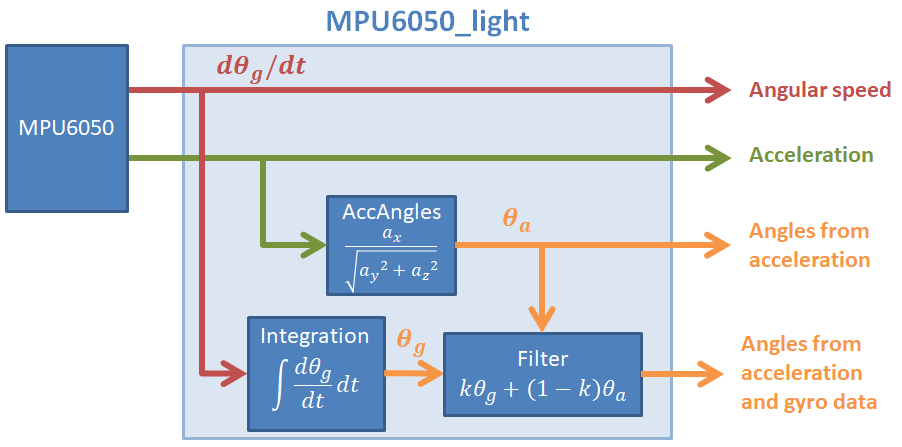
\includegraphics[width=1\textwidth]{Capitulo3 - Software/FiltroComplementar.png}\\
\caption{\label{fig:widgets}Operação do filtro - Imagem obtida na documentação da biblioteca "MPU6050\textunderscore light"}
\end{figure}

\section{Testes sem a estrutura 3D}

Durante o desenvolvimento do projeto foi utilizada uma aplicação web 3d para testes com sensor MPU-6050, que nos permitiu analisar seu funcionamento sem ter de acoplar motores ou quaisquer outros atuadores, tal aplicação é executada no navegador Chrome ou semelhante do computador, sendo necessário somente que o sensor esteja ligado a um arduino, e este arduino, ligado ao computador. Ao iniciar a aplicação, é solicitada a porta serial conectada ao sistema com o sensor, com isso, a interface fornece um cubo, como mostrado na figura 9, que acompanha a rotação do sensor no mundo real.

\begin{figure}[H]
\centering
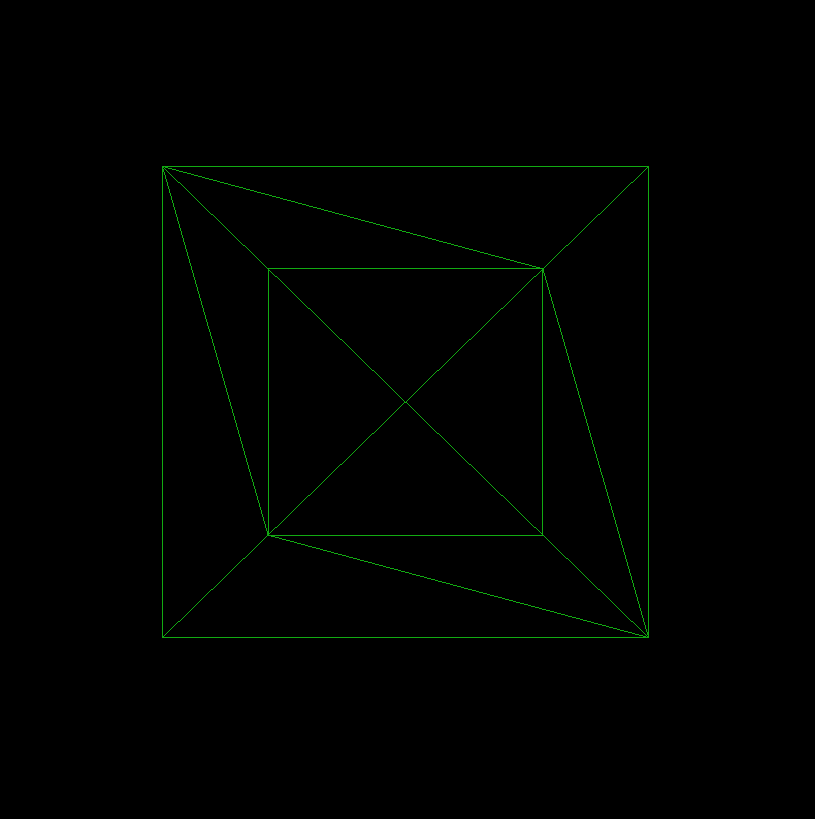
\includegraphics[width=0.6\textwidth]{Capitulo3 - Software/3dcubo.png}\\
\caption{\label{fig:widgets}Fluxograma da sequencia de operação do sistema.}
\end{figure}

\section{Leitura do Joystick}
No joystick é feito três leituras, o eixo x, eixo y e um botão de reset. Os eixos de movimento são lidos direto por portas analógicas no arduino e o botão por uma porta digital.\\
\indent O joystick controla um ajuste para cada eixo, esses ajustes são dois ângulos de desvio a ser considerados no posicionamento dos motores. Movendo um eixo do joystick para uma posição positiva o ajuste correspondente é incrementado com o tempo. O simétrico vale para uma posição negativa também. Podemos imaginar um plano "Ajuste X x Ajuste Y" com um ponto cujas as coordenadas são um ajuste final, o joystick então movimentaria esse ponto como se fosse um personagem de um jogo.

\pagebreak
\section{Controle dos servomotores}

Os servomotores são controlados por um sinal modulado por largura de pulso (PWM). O período do sinal é de 20ms e a largura de pulso varia entre 1ms e 2ms, que posicionam o servo nas posições 0º e 180º, respectivamente. Para poupar tempo de desenvolvimento foi utilizada a biblioteca "Servo" que gera essas formas de onda.\\
\indent Da saída do filtro complementar já temos um bom posicionamento, mas ainda causa solavancos extremos em quase todo movimento. Antes de enviar a nova posição de correção para os servos esse sinal ainda é tratado com um filtro de média levando em conta os últimos 5 valores e é adicionado o valor de ajuste do joystick. Então a posição do servomotor é interpolada entre a posição antiga e a nova posição corrigida. Dessa forma no começo de uma correção os motores se movimentam rapidamente e conforme se aproximam da posição final eles desaceleram, reduzindo os solavancos.